\documentclass[handout]{beamer}\usepackage[]{graphicx}\usepackage[]{color}
%% maxwidth is the original width if it is less than linewidth
%% otherwise use linewidth (to make sure the graphics do not exceed the margin)
\makeatletter
\def\maxwidth{ %
  \ifdim\Gin@nat@width>\linewidth
    \linewidth
  \else
    \Gin@nat@width
  \fi
}
\makeatother

\definecolor{fgcolor}{rgb}{0.345, 0.345, 0.345}
\newcommand{\hlnum}[1]{\textcolor[rgb]{0.686,0.059,0.569}{#1}}%
\newcommand{\hlstr}[1]{\textcolor[rgb]{0.192,0.494,0.8}{#1}}%
\newcommand{\hlcom}[1]{\textcolor[rgb]{0.678,0.584,0.686}{\textit{#1}}}%
\newcommand{\hlopt}[1]{\textcolor[rgb]{0,0,0}{#1}}%
\newcommand{\hlstd}[1]{\textcolor[rgb]{0.345,0.345,0.345}{#1}}%
\newcommand{\hlkwa}[1]{\textcolor[rgb]{0.161,0.373,0.58}{\textbf{#1}}}%
\newcommand{\hlkwb}[1]{\textcolor[rgb]{0.69,0.353,0.396}{#1}}%
\newcommand{\hlkwc}[1]{\textcolor[rgb]{0.333,0.667,0.333}{#1}}%
\newcommand{\hlkwd}[1]{\textcolor[rgb]{0.737,0.353,0.396}{\textbf{#1}}}%
\let\hlipl\hlkwb

\usepackage{framed}
\makeatletter
\newenvironment{kframe}{%
 \def\at@end@of@kframe{}%
 \ifinner\ifhmode%
  \def\at@end@of@kframe{\end{minipage}}%
  \begin{minipage}{\columnwidth}%
 \fi\fi%
 \def\FrameCommand##1{\hskip\@totalleftmargin \hskip-\fboxsep
 \colorbox{shadecolor}{##1}\hskip-\fboxsep
     % There is no \\@totalrightmargin, so:
     \hskip-\linewidth \hskip-\@totalleftmargin \hskip\columnwidth}%
 \MakeFramed {\advance\hsize-\width
   \@totalleftmargin\z@ \linewidth\hsize
   \@setminipage}}%
 {\par\unskip\endMakeFramed%
 \at@end@of@kframe}
\makeatother

\definecolor{shadecolor}{rgb}{.97, .97, .97}
\definecolor{messagecolor}{rgb}{0, 0, 0}
\definecolor{warningcolor}{rgb}{1, 0, 1}
\definecolor{errorcolor}{rgb}{1, 0, 0}
\newenvironment{knitrout}{}{} % an empty environment to be redefined in TeX

\usepackage{alltt}
%\documentclass{beamer}
\usepackage{graphicx}
\usepackage{amsmath,amssymb,array,comment,eucal}
\usepackage{xcolor}
\definecolor{beamer@blendedblue}{RGB}{86,155,189}
\definecolor{myblue}{RGB}{12,76,138}
\setbeamercolor{structure}{fg=myblue}
\definecolor{Ftitle}{RGB}{12,76,138}
\definecolor{Descitem}{RGB}{238,238,244}
\definecolor{StdTitle}{RGB}{12,76,138}
\definecolor{StdBody}{RGB}{213,24,0}
\definecolor{StdBody}{RGB}{213,24,0}

\definecolor{AlTitle}{RGB}{255, 190, 190}
\definecolor{AlBody}{RGB}{213,24,0}

\definecolor{ExTitle}{RGB}{201, 217, 217}
\definecolor{ExBody}{RGB}{213,24,0}

\setbeamercolor{frametitle}{fg = Ftitle}
\setbeamercolor{title}{fg = Ftitle}
\setbeamercolor{item}{fg = Ftitle}
\setbeamercolor{subitem}{fg = Ftitle}
\setbeamercolor{subsubitem}{fg = Ftitle}
\setbeamercolor{description item}{fg = myblue}
\setbeamercolor{titlelike}{fg=myblue}

%$Id: macros.tex,v 1.2 2006/02/13 14:23:55 rlw Exp rlw $
\newcommand{\Lmea}{{\cal L}} 
\newcommand{\scale}{\bflambda} 
\newcommand{\Scale}{\bfLambda} 
\newcommand{\bfscale}{\bflambda} 
\newcommand{\mean}{\bfchi}
\newcommand{\loc}{\bfchi}
\newcommand{\bfmean}{\bfchi}
\renewcommand{\k}{g}
\newcommand{\Gen}{{\cal G}}
\newcommand{\eps}{\epsilon}

\newcommand{\ind}{\mathrel{\mathop{\sim}\limits^{\mathit{ind}}}}
\newcommand{\iid}{\mathrel{\mathop{\sim}\limits^{\mathit{iid}}}}
\newcommand{\dis}{\mathrel{\mathop{=}\limits^{d}}}
\newcommand{\sgn}{\mathop{\rm sgn}}
\newcommand{\cmp}{h}
\newcommand{\dbdo}{d\beta ~ d\omega}
\newcommand{\real}{{\mathbb{R}}}
\newcommand{\Ber}{\mbox{\rm Ber}}
\newcommand{\GP}{\mbox{\rm GP}}
\newcommand{\SaS}{\text{S$\alpha$S}}
\newcommand{\RA}{{\real \times A}}
\newcommand{\RK}{{\real \times K}}
\newcommand{\RO}{{\real \times \Omega}} 
\newcommand{\RS}{{\bbR \times \LamS}}
  \newcommand{\set}[1]{\left\{#1\right\}}
  \newcommand{\bet}[1]{\left[#1\right]}
  \newcommand{\cet}[1]{\left(#1\right)}
%  \renewcommand{\half}{{\scriptstyle\frac12}}
\newcommand{\subA}{(\eps_1 < \beta \le \eps_2) \times \LamS}
 \newcommand{\uu}{{\big(\scale(x - \loc)\big)}}
 \newcommand{\uuj}{{\big(\scale_j(x-\loc_j)\big)}}
 \newcommand{\bbT}{{\mathbb{T}}}
 \newcommand{\ui}{{[0,1)}}
 \newcommand{\spq}[1]{\left|#1\right|^s_{pq}}
 \newcommand{\spqper}[1]{\left|#1\right|^{s\,*}_{pq}}
 \newcommand{\sspqper}[1]{\left\|#1\right\|^{s\,*}_{pq}}
 \newcommand{\sspq}[1]{\left\|#1\right\|^s_{pq}}    % Besov semi-norm
 \newcommand{\qp}[1]  {\left\|#1\right\|^q_p}         % Hilbert-space norm
 \newcommand{\qper}[1]{\left\|#1\right\|^{*\,q}_p}  % Periodic HS norm
 

\newcommand{\bbW}{{\mathbb{W}}}
\newcommand{\bbB}{{\mathbb{B}}}
\newcommand{\Sob}{{\ensuremath{\bbW^s_2}}}
\newcommand{\Besov}{{\ensuremath{\bbB^s_{pq}}}}
\newcommand{\Besper}{{\ensuremath{\bbB^{s\,*}_{pq}}}}
\newcommand{\Sobx}[1]{{\bbW^{#1}_2}}
\newcommand{\Besovx}[1]{{\bbB^{#1}_2}}
\newcommand{\SN}[1]{\|{#1}\|_\Sob}
% MATH LETTER DEFINITIONS
\newcommand{\Levy}{L{\'e}vy}
\newcommand{\nmathbf}{\bm}
\newcommand{\tabb}[1]{\hspace*{#1\parindent}}
%\newcommand{\G}{{g}}    % Really the same as \GB
\newcommand{\g}{{\phi}} %\newcommand{\g}{{g}}
\newcommand{\GB}{{g}}  
% Roman math Bold face 


\def\bfA{\nmathbf A}
\def\bfB{\nmathbf B}
\def\bfC{\nmathbf C}
\def\bfD{\nmathbf D}
\def\bfE{\nmathbf E}
\def\bfF{\nmathbf F}
\def\bfG{\nmathbf G}
\def\bfH{\nmathbf H}
\def\bfI{\nmathbf I}
\def\bfJ{\nmathbf J}
\def\bfK{\nmathbf K}
\def\bfL{\nmathbf L}
\def\bfM{\nmathbf M}
\def\bfN{\nmathbf N}
\def\bfO{\nmathbf O}
\def\bfP{\nmathbf P}
\def\bfQ{\nmathbf Q}
\def\bfR{\nmathbf R}
\def\bfS{\nmathbf S}
\def\bfT{\nmathbf T}
\def\bfU{\nmathbf U}
\def\bfV{\nmathbf V}
\def\bfW{\nmathbf W}
\def\bfX{\nmathbf X}
\def\bfY{\nmathbf Y}
\def\bfZ{\nmathbf Z}

\def\bfa{\nmathbf a}
\def\bfb{\nmathbf b}
\def\bfc{\nmathbf c}
\def\bfd{\nmathbf d}
\def\bfe{\nmathbf e}
\def\bff{\nmathbf f}
\def\bfg{\nmathbf g}
\def\bfh{\nmathbf h}
\def\bfi{\nmathbf i}
\def\bfj{\nmathbf j}
\def\bfk{\nmathbf k}
\def\bfl{\nmathbf l}
\def\bfm{\nmathbf m}
\def\bfn{\nmathbf n}
\def\bfo{\nmathbf o}
\def\bfp{\nmathbf p}
\def\bfq{\nmathbf q}
\def\bfr{\nmathbf r}
\def\bfs{\nmathbf s}
\def\bft{\nmathbf t}
\def\bfu{\nmathbf u}
\def\bfv{\nmathbf v}
\def\bfw{\nmathbf w}
\def\bfx{\nmathbf x}
\def\bfy{\nmathbf y}
\def\bfz{\nmathbf z}


\def\bfalpha  {\nmathbf \alpha}
\def\bfbeta   {\nmathbf \beta}
\def\bfgamma  {\nmathbf \gamma}
\def\bfdelta  {\nmathbf \delta}
\def\bfepsilon{\nmathbf \epsilon}
\def\bfvareps {\nmathbf \varepsilon}
\def\bfzeta   {\nmathbf \zeta}
\def\bfeta    {\nmathbf \eta}
\def\bftheta  {\nmathbf \theta}
\def\bfiota   {\nmathbf \iota}
\def\bfkappa  {\nmathbf \kappa}
\def\bflambda {\nmathbf \lambda}
\def\bfmu     {\nmathbf \mu}
\def\bfnu     {\nmathbf \nu}
\def\bfxi     {\nmathbf \xi}
\def\bfomicron{\nmathbf \omicron}
\def\bfpi     {\nmathbf \pi}
\def\bfrho    {\nmathbf \rho}
\def\bfsigma  {\nmathbf \sigma}
\def\bftau    {\nmathbf \tau}
\def\bfupsilon{\nmathbf \upsilon}
\def\bfphi    {\nmathbf \phi}
\def\bfpsi    {\nmathbf \psi}
\def\bfchi    {\nmathbf \chi}
\def\bfomega  {\nmathbf \omega}
\newcommand{\nubw}{{\tilde\nu}}  % no longer red!
\def\bfAlpha  {\nmathbf \Alpha}
\def\bfBeta   {\nmathbf \Beta}
\def\bfGamma  {\nmathbf \Gamma}
\def\bfDelta  {\nmathbf \Delta}
\def\bfEpsilon{\nmathbf \Epsilon}
\def\bfZeta   {\nmathbf \Zeta}
\def\bfEta    {\nmathbf \Eta}
\def\bfTheta  {\nmathbf \Theta}
\def\bfIota   {\nmathbf \Iota}
\def\bfKappa  {\nmathbf \Kappa}
\def\bfLambda {\nmathbf \Lambda}
\def\bfMu     {\nmathbf \Mu}
\def\bfNu     {\nmathbf \Nu}
\def\bfXi     {\nmathbf \Xi}
\def\bfOmicron{\nmathbf \Omicron}
\def\bfPi     {\nmathbf \Pi}
\def\bfRho    {\nmathbf \Rho}
\def\bfSigma  {\nmathbf \Sigma}
\def\bfTau    {\nmathbf \Tau}
\def\bfUpsilon{\nmathbf \Upsilon}
\def\bfPhi    {\nmathbf \Phi}
\def\bfPsi    {\nmathbf \Psi}
\def\bfChi    {\nmathbf \Chi}
\def\bfOmega  {\nmathbf \Omega}

% Number math Bold face

\newcommand{\bfzero}{{\nmathbf 0}}
\newcommand{\bfone}{{\nmathbf 1}}

% Estimators

\newcommand{\ttheta}{\tilde{\theta}}
\newcommand{\htheta}{\hat{\theta}}
\newcommand{\tbtheta}{\tilde{\bftheta}}
\newcommand{\hbtheta}{\hat{\bftheta}}
\newcommand{\tomega}{\tilde{\omega}}
\newcommand{\homega}{\hat{\omega}}
\newcommand{\tbomega}{\tilde{\bfomega}}
\newcommand{\hbomega}{\hat{\bfomega}}
\newcommand{\tlambda}{\tilde{\lambda}}
\newcommand{\hlambda}{\hat{\lambda}}
\newcommand{\tblambda}{\tilde{\bflambda}}
\newcommand{\hblambda}{\hat{\bflambda}}


% Calligraphic

\newcommand{\mc}[1]{\ensuremath{\mathcal{#1}}}

\newcommand{\cfA}{\mc{A}}
\newcommand{\cfB}{\mc{B}}
\newcommand{\cfC}{\mc{C}}
\newcommand{\cfD}{\mc{D}}
\newcommand{\cfE}{\mc{E}}
\newcommand{\cfF}{\mc{F}}
\newcommand{\cfG}{\mc{G}}
\newcommand{\cfH}{\mc{H}}
\newcommand{\cfI}{\mc{I}}
\newcommand{\cfJ}{\mc{J}}
\newcommand{\cfK}{\mc{K}}
\newcommand{\cfL}{\mc{L}}
\newcommand{\cfM}{\mc{M}}
\newcommand{\cfN}{\mc{N}}
\newcommand{\cfO}{\mc{O}}
\newcommand{\cfP}{\mc{P}}
\newcommand{\cfQ}{\mc{Q}}
\newcommand{\cfR}{\mc{R}}
\newcommand{\cfS}{\mc{S}}
\newcommand{\cfT}{\mc{T}}
\newcommand{\cfU}{\mc{U}}
\newcommand{\cfV}{\mc{V}}
\newcommand{\cfX}{\mc{X}}
\newcommand{\cfY}{\mc{Y}}
\newcommand{\cfZ}{\mc{Z}}

\newcommand{\bmc}[1]{\ensuremath{\boldsymbol{\mathcal{#1}}}}

\newcommand{\bcfA}{\bmc{A}}
\newcommand{\bcfB}{\bmc{B}}
\newcommand{\bcfC}{\bmc{C}}
\newcommand{\bcfD}{\bmc{D}}
\newcommand{\bcfE}{\bmc{E}}
\newcommand{\bcfF}{\bmc{F}}
\newcommand{\bcfG}{\bmc{G}}
\newcommand{\bcfH}{\bmc{H}}
\newcommand{\bcfI}{\bmc{I}}
\newcommand{\bcfJ}{\bmc{J}}
\newcommand{\bcfK}{\bmc{K}}
\newcommand{\bcfL}{\bmc{L}}
\newcommand{\bcfM}{\bmc{M}}
\newcommand{\bcfN}{\bmc{N}}
\newcommand{\bcfO}{\bmc{O}}
\newcommand{\bcfP}{\bmc{P}}
\newcommand{\bcfQ}{\bmc{Q}}
\newcommand{\bcfR}{\bmc{R}}
\newcommand{\bcfS}{\bmc{S}}
\newcommand{\bcfT}{\bmc{T}}
\newcommand{\bcfU}{\bmc{U}}
\newcommand{\bcfV}{\bmc{V}}
\newcommand{\bcfW}{\bmc{W}}
\newcommand{\bcfX}{\bmc{X}}
\newcommand{\bcfY}{\bmc{Y}}
\newcommand{\bcfZ}{\bmc{Z}}

% Special symbols

\newcommand{\reals}{\mbox{\rm I\kern-.20em R}}
\newcommand{\sreals}{\mbox{\small \rm I\kern-.20em R}}
\newcommand{\LamS}{{\cS^d_+}}

% MATHEMATICAL NOTATION

% Operators

\newcommand{\bg}{\;\bigg\vert\;}
\newcommand{\pr}{\mbox{\rm Pr}}
\newcommand{\D}{\mbox{\rm D}}
\newcommand{\E}{\mbox{\rm E}}
\newcommand{\Mo}{\mbox{\rm Mo}}
\newcommand{\Me}{\mbox{\rm Me}}
\newcommand{\Cov}{\mbox{\rm Cov}}
\newcommand{\Var}{\mbox{\rm Var}}
\newcommand{\Corr}{\mbox{\rm Corr}}
\newcommand{\Q}{\mbox{\rm Q}}

% Distributions
\newcommand{\BeBi}{\mbox{\rm BeBi}}
\newcommand{\Be}{\mbox{\rm Be}}
\newcommand{\Bi}{\mbox{\rm Bi}}
\newcommand{\Br}{\mbox{\rm Br}}
\newcommand{\Ca}{\mbox{\rm Ca}}
\newcommand{\Di}{\mbox{\rm Di}}
\newcommand{\Ex}{\mbox{\rm Ex}}
\newcommand{\Fs}{\mbox{\rm Fs}}
\newcommand{\Ga}{\mbox{\sf G}}
\newcommand{\Ge}{\mbox{\rm Ge}}
\newcommand{\GaGa}{\mbox{\rm GaGa}}
\newcommand{\Hy}{\mbox{\rm Hy}}
\newcommand{\IGa}{\mbox{\rm IGa}}
\newcommand{\IPa}{\mbox{\rm IPa}}
\newcommand{\Lo}{\mbox{\rm Lo}}
\newcommand{\Mu}{\mbox{\rm Mu}}
\newcommand{\N}{\mbox{\rm N}}
\newcommand{\NBi}{\mbox{\rm NBi}}
\newcommand{\NGa}{\mbox{\rm NGa}}
\newcommand{\NWi}{\mbox{\rm NWi}}
\newcommand{\Pa}{\mbox{\rm Pa}}
\newcommand{\Po}{\mbox{\sf P}}
\newcommand{\PoGa}{\mbox{\rm PoGa}}
\newcommand{\Ra}{\mbox{\rm Ra}}
\newcommand{\REx}{\mbox{\rm REx}}
\newcommand{\St}{\mbox{\rm St}}
\newcommand{\Un}{\mbox{\rm Un}}
\newcommand{\Wi}{\mbox{\rm Wi}}

% General Mathematics

\newcommand{\dd}[1]{\,d{#1}}
\newcommand{\barx}{\ensuremath{\bar{x}}}
\newcommand{\comb}[2]{{#1\choose#2}}
\newcommand{\ontop}[2]{{#1\atop#2}}
\newcommand{\h}{{\small\ensuremath{1\over2}}}
\newcommand{\hh}[2]{{\small\ensuremath{#1\over#2}}}

\newcommand{\fn}[1]{\hbox{\textrm{#1}}}
\newcommand{\cred}{\fn{Cr}}
\newcommand\dlim{\mathop{\rm \hbox{$\delta$}lim}}
\newcommand{\goto}{\rightarrow}
\newcommand{\gotoinf}{\rightarrow \infty}

\newcommand{\data}{\ensuremath{\bfx=\{x_1,\ldots,x_n\}}}
\newcommand{\brow}[2]{\ensuremath{\{{#1}_1,\ldots,{#1}_{#2}\}}}
\newcommand{\prow}[2]{\ensuremath{({#1}_1,\ldots,{#1}_{#2})}}

\newcommand{\met}{\thinspace{\rm m}}\newcommand{\km}{\thinspace{\rm km}}
\newcommand{\xbar}{\overline X}%
\newcommand{\xbbar}{\overline{\overline X}}%
\font\ss=cmss12
 \newcommand{\OFP}{(\Omega,\cF,\P)}
 \newcommand{\bbC}{\mathbb{C}}
 \newcommand{\bbF}{\mathbb{F}}
 \newcommand{\bbN}{\mathbb{N}}
 \newcommand{\bbR}{\mathbb{R}}
 \newcommand{\bbX}{\mathbb{X}}
 \newcommand{\bbZ}{\mathbb{Z}}
 \newcommand{\one}[1]{\mathbf{1}_{\{#1\}}}
 \newcommand{\cA}{{\cal A}}
 \newcommand{\cB}{{\cal B}} 
 \newcommand{\cE}{{\cal E}}
 \newcommand{\cF}{{\cal F}}
 \newcommand{\cG}{{\cal G}}
 \newcommand{\cH}{{\cal H}}
 \newcommand{\cM}{{\cal M}}
 \newcommand{\cR}{{\cal R}}
 \newcommand{\cS}{{\cal S}}
 \newcommand{\cT}{{\cal T}}
 \newcommand{\cX}{{\cal X}}
 \newcommand{\cY}{{\cal Y}}
 \newcommand{\cZ}{{\cal Z}}
 \newcommand{\eF}{{\CMcal F}}
 \newcommand{\eG}{{\CMcal G}} 
 \newcommand{\eH}{{\CMcal H}}
 \renewcommand{\P}{{\sf{P}}} 
 \renewcommand{\E}{{\sf{E}}}
 \newcommand{\Ev}{{\sf{Ev}}}%
 \newcommand{\V}{{\sf{V}}} 
 \renewcommand{\Cov}{{\sf{Cov}}}
 %\newcommand{\Be}{\textsf{Be}}
 %\newcommand{\Bi}{\textsf{Bi}}
 %\newcommand{\Ex}{\textsf{Ex}}\newcommand{\Ga}{\textsf{Ga}}
 %\newcommand{\Di}{\textsf{Di}}\newcommand{\Ge}{\textsf{Ge}}
 %\newcommand{\IG}{\textsf{IG}}\newcommand{\Lv}{\textsf{Lv}}
 %\newcommand{\HG}{\textsf{HG}}\newcommand{\MN}{\textsf{MN}}
\newcommand{\NB}{\textsf{NB}}\newcommand{\No}{\textsf{N}}
\newcommand{\LN}{\textsf{LN}}
\newcommand{\Lv}{\mbox{\rm Lv}}
%\newcommand{\Pa}{\textsf{Pa}}
% \newcommand{\Po}{\textsf{Po}}\newcommand{\Un}{\textsf{Un}}
 \newcommand{\argmax}{\textrm{argmax}}
 \renewcommand{\th}{{\ensuremath^{\mbox{\tiny th}}}}
 \newcommand{\nd}{{\ensuremath^{\mbox{\tiny nd}}}}
 \newcommand{\st}{{\ensuremath^{\mbox{\tiny st}}}}
 \newcommand{\ii}{{\ensuremath{\bar{i}}}}% \newcommand{\ii}{{\hat i}}
 \newcommand{\jj}{{\ensuremath{\bar{j}}}}%
 \newcommand{\R}{\texttt{R}}
 \newcommand{\mayeq}{\mathrel{\mathop{=}\limits^?}}
 \newcommand{\pperp}{\mathrel{{\rlap{$~\perp$}\perp\,\,}}}
 \newbox\asbox
 \setbox\asbox=\hbox{\vrule height 15pt depth3.5pt width0pt}
 \def\astrut{\relax\ifmmode\copy\strutbox\else\unhcopy\strutbox\fi}
 \def\Strut{\vrule width0pt height 16pt depth 4pt}%
%\font\tinyss=cmss8 at 8truept % for ^T etc
\newcommand{\tsf}[1]{\textsf{\tiny{#1}}}
\newcommand{\fxa}{\mbox{$f(x\mid\alpha)$}}
\newcommand{\fxt}{\mbox{$f(x\mid\theta)$}}
\newcommand{\fxat}{\mbox{$f(x\mid\alpha,\theta)$}}
\newcommand{\tp}{^{\tsf{T}}}
\newcommand{\as}{\textit{a.s.}}
\newcommand{\ie}{\textit{i.e.{}}}
\newcommand{\etc}{\textit{etc}}
\newcommand{\eg}{\textit{e.g.{}}}%
\newcommand{\half}{{\frac12}}
\newcommand{\Sec}[1]{Section\thinspace(\ref{#1})}
\newcommand{\Thm}[1]{Theorem\thinspace\ref{#1}}
\newcommand{\Cor}[1]{Corollary\thinspace\ref{#1}}
\newcommand{\Eqn}[1]{Equation\thinspace(\ref{#1})}
\newcommand{\Fig}[1]{Figure\thinspace(\ref{#1})}
\newcommand{\Figs}[2]{Figures\thinspace(\ref{#1}) and (\ref{#2})}
\newcommand{\Figab}[2]{Figure\thinspace(\ref{#1}#2)}
\newcommand{\Tab}[1]{Table\thinspace(\ref{#1})}
\newcommand{\jth}{{\ensuremath j^{\mbox{\tiny th}}}}%
\providecommand{\ij}{_{ij}} \newcommand{\ji}[1]{_{ij#1}}%
\newcount\ola \newcount\olb \newcount\olc \newcount\old \newcount\ole
\newcount\och\newcount\level
\newtheorem{cor}{Corollary}
\newtheorem{define}{Definition}
\newtheorem{lem}{Lemma}
\newtheorem{prob}{Problem}
\newtheorem{prop}{Proposition}
\newtheorem{thm}{Theorem}
\def\OL#1{\par\noindent\hangindent=#1\parindent % Outline
  \kern1\hangindent\ignorespaces}%
\def\ol#1{%
    \level=#1
    \ifcase\level
    \ola=0 \olb=0 \olc=0 \old=0 \ole=0\or         % Level 0 (reset)
    \olb=0 \olc=0 \old=0 \ole=0 \advance\ola by 1 % Level 1
    \gdef\olev{\uppercase\expandafter{\romannumeral\ola}} \or
    \olc=0 \old=0 \ole=0 \advance\olb by 1        % Level 2
    \och=64 \advance\och by\olb
    \gdef\olev{\char\och}\or
    \old=0 \ole=0 \advance\olc by 1               % Level 3
    \och=48 \advance\och by\olc
    \gdef\olev{\char\och}\or
    \ole=0 \advance\old by 1                      % Level 4
    \och=96 \advance\och by\old
    \gdef\olev{\char\och}\or
    \advance\ole by 1                             % Level 5
    \gdef\olev{\romannumeral\ole} \or
    \message{Outline depth too deep: #1}\fi
    \ifnum\level>0 \OL\level\llap{\olev.\enspace}\ignorespaces\fi}%
\long\def\comment#1/*#2*/{\endcomment}%
\def\endcomment{\relax}%
%
\makeatletter % Find hours (count1) and minutes (count2) past midnight:
\count1\time \divide\count1 60 \count2=-\count1
\multiply\count2 60 \advance\count2 \time
\edef\now{\two@digits{\the\count1}:\two@digits{\the\count2}}
%\renewcommand\section{\@startsection     % Smaller and sans-serif
%    {section}{1}{\z@}{-3.5ex \@plus -1ex \@minus -.2ex}%
%    {2.3ex \@plus.2ex}{\normalfont\large\bfseries\sffamily}}
%\renewcommand\subsection{\@startsection
%    {subsection}{2}{\z@}{-3.25ex\@plus -1ex \@minus -.2ex}%
%    {1.5ex \@plus .2ex}{\normalfont\large\bfseries\sffamily}}
%\renewcommand\subsubsection{\@startsection
%    {subsubsection}{3}{\z@}{-3.25ex\@plus -1ex \@minus -.2ex}%
%    {1.5ex \@plus .2ex}{\normalfont\normalsize\bfseries\sffamily}}
%\def\@seccntformat#1{\csname the#1\endcsname.\quad} % Add . to sec num's
%\long\def\@makecaption#1#2{%                          Use . not : in cap'ns
%  \vskip\abovecaptionskip
%  \sbox\@tempboxa{#1. #2}%
%  \ifdim \wd\@tempboxa >\hsize
%    #1. #2\par
%  \else
%    \global \@minipagefalse
%    \hb@xt@\hsize{\hfil\box\@tempboxa\hfil}%
%  \fi
%  \vskip\belowcaptionskip}
% BEAMER FIX START
\def\newblock{\beamer@newblock}
% BEAMER FIX END
\makeatother

\def\wbox#1#2#3{{\vcenter{\vbox{\hrule height.#3pt
    \hbox{\vrule width.#3pt height#1pt \kern#2pt \vrule width.#3pt}%
                            \hrule height.#3pt}}}}%
\def\Proof.{\medbreak\noindent{\bf Proof.\enspace}}
\def\qed{{\nobreak\hfill\penalty0\hbox to1truecm{}\nobreak
    \hfill$\wbox634$\par\bigskip}}%



%\usetheme{Warsaw}
%\usecolortheme{orchid}
\title{Bayesian Estimation in Linear Models \& Choice of Prior Distributions}
\institute{Merlise Clyde}
\author{STA521 Predicitve Models Duke University}
\date{\today}
\IfFileExists{upquote.sty}{\usepackage{upquote}}{}
\begin{document}
\maketitle

\begin{frame} \frametitle{Bayesian Estimation}
  Model $\Y = \X \b + \eps$  with $\eps \sim \N(\zero_n , \sigma^2
  \I_n)$ \pause
is equivalent to
$$
\Y \sim \N(\X \b, \I_n/\phi)
$$
\pause
 $\phi = 1/\sigma^2$ is the {\it precision}.
\pause

\vspace{14pt}
In the  Bayesian paradigm describe uncertainty about unknown
parameters using probability distributions
\pause
\begin{itemize}
\item  Prior Distribution $p(\b, \phi)$ describes uncertainty about
  parameters prior to seeing the data \pause
\item Posterior Distribution $p(\b, \phi \mid \Y)$ describes
  uncertainty about the parameters after updating  beliefs given the
  observed data \pause
\item updating rule is based on Bayes Theorem
$$p(\b, \phi \mid \Y) \propto \cL(\b, \phi) p(\b, \phi)$$
\pause
\end{itemize}
 reweight prior beliefs by likelihood of parameters  under observed data
\end{frame}


\begin{frame} \frametitle{Prior Distributions}
Factor joint prior distribution  $$p(\b, \phi) = p(\b \mid \phi) p(\phi)$$
\pause

Convenient choice is to take ``Conjugate'' family \pause
\begin{itemize}
\item $\b \mid \phi \sim \N(b_0, \Phi_0^{-1}/\phi)$ where $b_0$ is the prior
  mean and $\Phi^{-1}/\phi$ is the prior covariance of $\b$
$$
p(\b \mid \phi) = \frac{1}{(2 \pi)^{p/2}} | \phi \Phi_0|^{1/2} e^{- \frac{1}{2}\phi (\b - \bv_0)^T \Phi_0 (\b - \bv_0)}
$$
\pause
\item $\phi \sim \G( \nu_0/2, \SS_0/2)$  with $\E(\sigma^2) =
  \SS_0/(\nu_0 - 2)$ \pause
$$p(\phi) = \frac{1}{\Gamma{(\nu_0/2)}}
\left(\frac{\SS_0}{2} \right)^{\nu_0/2}
\phi^{\nu_0/2 - 1}
 e^{- \phi \SS_0/2}
 $$\pause
\item $(\b, \phi)^T \sim \NG(\bv_0, \Phi_0, \nu_0, \SS_0)$ \pause
\item Conjugate  ``Normal-Gamma'' family implies \pause
$$(\b, \phi)^T \mid \Y \sim \NG(\bv_n, \Phi_n, \nu_n, \SS_n)$$
\end{itemize}
\end{frame}

\begin{frame}
\frametitle{Finding the Posterior Distribution}
Express Likelihood: $\cL(\beta, \phi) \propto \phi^{n/2} e^{- \phi \frac{\SSE}{2}}
e^{-\frac{\phi}{2} (\b - \bhat)^T(\X^T\X) (\b - \bhat)}$ \pause
\begin{eqnarray*}
 p(\b, \phi \mid \Y) &\propto&  \phi^{\frac {n + p + \nu_0}{ 2} - 1}
 e^{- \frac \phi 2 ( \SSE + \SS_0) } \\
 & & e^{-\frac{\phi}{2} (\b - \bhat)^T(\X^T\X) (\b - \bhat)}
 e^{- \frac{\phi}{2} (\b - \bv_0)^T \Phi (\b - \bv_0) }
\end{eqnarray*} \pause


\end{frame}


\begin{frame}
\frametitle{Finding the Posterior Distribution}
\begin{eqnarray*}
 p(\b, \phi \mid \Y) &\propto&  \phi^{\frac {n + p + \nu_0}{ 2} - 1}
 e^{- \frac \phi 2 ( \SSE + \SS_0) } \\
 & & e^{-\frac{\phi}{2} (\b - \bhat)^T(\X^T\X) (\b - \bhat)}
 e^{- \frac{\phi}{2} (\b - \bv_0)^T \Phi (\b - \bv_0) }
\end{eqnarray*} \pause

Quadratic in Normal
$$\exp\left\{- \frac{\phi}{2} (\b - \bv)^T \Phi (\b - \bv) \right\} = \exp\left\{-
  \frac{\phi}{2} (\b^T \Phi \b - 2 \b^T \Phi \bv + \bv^T\Phi \bv )\right\}$$
\pause

  \begin{itemize}
  \item Expand quadratics and regroup terms \pause
  \item Read off posterior precision from Quadratic in $\b$ \pause
  \item Read off posterior mean from Linear term in $\b$ \pause
  \item will need to complete the quadratic in the posterior mean
  \end{itemize}
\end{frame}


\begin{frame}  \frametitle{ Expand and Regroup}
  Quadratic in Normal
$$\exp\left\{- \frac{\phi}{2} (\b - \bv)^T \Phi (\b - \bv) \right\} = \exp\left\{-
  \frac{\phi}{2} (\b^T \Phi \b - 2 \b^T \Phi \bv + \bv^T\Phi \bv )\right\}$$
\pause

\begin{eqnarray*}
 p(\b, \phi \mid \Y) &\propto&  \phi^{\frac {n + p + \nu_0}{ 2} - 1}
 e^{- \frac \phi 2 ( \SSE + \SS_0) }  \\
 & & e^{-\frac{\phi}{2} (\b - \bhat)^T(\X^T\X) (\b - \bhat)}
 e^{- \frac{\phi}{2} (\b - \bv_0)^T \Phi_0 (\b - \bv_0) } \pause  \\
 & = & \phi^{\frac {n + p + \nu_0}{ 2} - 1}
 e^{- \frac \phi 2 ( \SSE + \SS_0) } \pause \\
& &  e^{ -\frac{\phi}{2} \left(  \b^T (\X^T\X + \Phi_0) \b  \right) } \pause \\
& &  e^{  -\frac{\phi}{2} \left( -2 \b^T (\X^T\X \bhat  + \Phi_0 \bv_0)
   \right)} \pause \\
& &  e^{  -\frac{\phi}{2} (\bhat^T \X^T\X \bhat + \bv_0^T \Phi_0 \bv_0
  )}
\end{eqnarray*}


\end{frame}

\begin{frame} \frametitle{ Identify Hyperparameters and Complete the Quadratic}
  Quadratic in Normal
$$\exp\left\{- \frac{\phi}{2} (\b - \bv)^T \Phi (\b - \bv) \right\} = \exp\left\{-
  \frac{\phi}{2} (\b^T \Phi \b - 2 \b^T \Phi \bv + \bv^T\Phi \bv )\right\}$$
\pause


Let $\Phi_n = \X^T\X + \Phi_0$ \pause
  \begin{eqnarray*}
 p(\b, \phi \mid \Y) &\propto&  \phi^{\frac {n + p + \nu_0}{ 2} - 1}
 e^{- \frac \phi 2 ( \SSE + \SS_0) } \pause \\
& &  e^{ -\frac{\phi}{2} \left(  \b^T \alert<4>{(\X^T\X + \Phi_0)} \b
  \right) } \pause\\
& &  e^{  -\frac{\phi}{2} \left( -2 \b^T \alert<5>{\Phi_n \Phi_n^{-1}} (\X^T\X \bhat  + \Phi_0 \bv_0)
   \right)} \pause\\
& &  e^{ -\frac{\phi}{2} (\alert<6>{\bv_ n^T \Phi_n \bv_n - \bv_n^T \Phi_0
  \bv_n}) } \pause \\
& &  e^{  -\frac{\phi}{2} (\bhat^T \X^T\X \bhat + \bv_0^T \Phi_0 \bv_0
  )} \pause \\
& = &
  \phi^{\frac {n + p+  \nu_0}{ 2} - 1}
 e^{- \frac \phi 2 ( \SSE + \SS_0  + \bhat^T \X^T\X \bhat + \bv_0^T \Phi_0 \bv_0
 - \bv_n^T \Phi_n \bv_n)}  \pause  \\
& &  e^{ -\frac{\phi}{2} \left(  \b^T \alert{(\Phi_n)} \b
  \right) } \pause\\
& &  e^{  -\frac{\phi}{2} \left( -2 \b^T \Phi_n\alert{\Phi_n^{-1} (\X^T\X \bhat  + \Phi_0 \bv_0)}
   \right)} \pause\\
& &  e^{ -\frac{\phi}{2} (\alert{\bv_ n^T \Phi_n \bv_n}) }
  \end{eqnarray*}

\end{frame}


\begin{frame} \frametitle{Posterior Distribution}
  \begin{eqnarray*}
 p(\b, \phi \mid \Y) &\propto&
  \phi^{\frac {n +  \nu_0}{ 2} - 1}
 e^{- \frac \phi 2 ( \SSE + \SS_0  + \bhat^T \X^T\X \bhat + \bv_0^T \Phi_0 \bv_0
 - \bv_n^T \Phi_n \bv_n)} \\
& & \phi^{\frac p 2} e^{- \frac{\phi}{2} (\b - \bv_n)^T \Phi_n (\b -
  \bv_n) }  \pause  \\
& & \\
\Phi_n & = & \X^T\X +  \Phi_0 \pause \\
\bv_n &  = & \Phi_n^{-1} (\X^T\X \bhat  + \Phi_0 \bv_0) \pause
  \end{eqnarray*}

Posterior Distribution
  \begin{eqnarray*}
\b \mid \phi, \Y & \sim &\N(\bv_n, (\phi \Phi_n)^{-1}) \pause \\
\phi \mid \Y &\sim &\G(\frac{n + \nu_0}{2}, \frac{\SSE + \SS_0 + \bhat^T \X^T\X \bhat + \bv_0^T \Phi_0 \bv_0
 - \bv_n^T \Phi_n \bv_n}{2})
  \end{eqnarray*}


\end{frame}



\begin{frame}
  \frametitle{Predictive Distribution}
Suppose $\Y^* \mid \b, \phi \sim \N(\X^* \b , \I/\phi)$  and is conditionally
independent of $\Y$ given $\b$ and $\phi$ \pause
\vspace{18pt}

What is the predictive distribution of $\Y^* \mid \Y$? \pause

\vspace{18pt}
$\Y^* = \X^* \b + \eps^*$ and $\eps^*$ is independent of $\Y$ given
$\phi$ \pause

\begin{eqnarray*}
\X^* \b + \eps^* \mid \phi, \Y & \sim & \N(\X^*\bv_n, (\X^{*} \Phi_n^{-1} \X^{*T}
+ \I)/\phi)  \pause \\
\Y^* \mid \phi, \Y & \sim & \N(\X^*\bv_n, (\X^{*} \Phi_n^{-1} \X^{*T}
+ \I)/\phi)  \pause \\
\phi \mid \Y & \sim & \G\left(\frac{\nu_n}{2},
  \frac{\shat \nu_n}{ 2} \right)  \pause \\
\Y^* \mid \Y & \sim & t_{\nu_n}( \X^*\bv_n, \shat (\I + \X^* \Phi_n^{-1} \X^T))
\end{eqnarray*}
\end{frame}
\begin{frame}
  \frametitle{Alternative Derivation}
Conditional Distribution:
\begin{eqnarray*}
f(\Y^* \mid \Y) & = & \frac{f(\Y^*, \Y)}{f(\Y)} \pause \\
 & = & \frac{
\iint f(\Y^*, \Y \mid \b, \phi) p(\b, \phi) d\b\, d\phi
}
{
  f(\Y)
}  \pause \\
 & = & \frac{
\iint f(\Y^*\mid \b, \phi) f(\Y \mid \b, \phi) p(\b, \phi) d\b\, d\phi
}
{
  f(\Y)
}  \pause \\
 & = &
\iint f(\Y^*\mid \b, \phi)  p(\b, \phi \mid \Y) d\b\, d\phi \pause
\end{eqnarray*}
\end{frame}

\begin{frame}
  \frametitle{Conjugate Priors}
  \begin{definition}
    A class of prior distributions $\cP$ for $\t$ is conjugate for a
    sampling model $p(y \mid \t)$ if for every $p(\t) \in \cP$, $p(\t
    \mid \Y) \in \cP$.
  \end{definition}
\pause
  Advantages: \pause
  \begin{itemize}
  \item Closed form distributions for most quantities; bypass Monte Carlo for
    calculations \pause
  \item Simple updating in terms of sufficient statistics ``weighted
    average'' - useful with big data \pause
  \item Interpretation as prior samples - prior sample size \pause
  \item Elicitation of prior through imaginary or historical data \pause
  \item limiting ``non-proper'' form recovers MLEs \pause
  \end{itemize}
Choice of conjugate prior?
\end{frame}

\begin{frame}
  \frametitle{Unit Information Prior}

Unit information prior $\b \mid \phi \sim \N(\bhat, n
   (\X^T\X)^{-1}/\phi)$ \pause
  \begin{itemize}
\item Fisher Information is $\phi \X^T\X$ based on a sample of $n$
  observations \pause
\item Inverse Fisher information is covariance matrix of MLE \pause
\item ``average information'' in one observation is  $\phi \X^T\X /n$ \pause
\item center prior at MLE and base covariance on the information in
  ``1'' observation \pause
\item  Posterior mean
$$\frac{n}{1 + n} \bhat +  \frac{1}{1 + n}\bhat = \bhat$$ \pause
\item Posterior Distribution
$$\b \mid \Y, \phi \sim \N\left( \bhat, \frac{n}{1 + n} (\X^T\X)^{-1}
  \phi^{-1} \right)$$ \pause
    \end{itemize}
Cannot represent real prior beliefs; double use of data
\end{frame}

\begin{frame}
  \frametitle{Zellner's $g$-prior}
Zellner's g-prior(s) $\b \mid \phi \sim \N(\bv_0, g
    (\X^T\X)^{-1}/\phi)$ \pause

$$\b \mid \Y, \phi \sim \N\left( \frac{g}{1 + g} \bhat +  \frac{1}{1 + g}
\bv_0, \frac{g}{1 + g} (\X^T\X)^{-1} \phi^{-1} \right)$$ \pause

\begin{itemize}
\item Zellner proposed informative choice for the prior mean
\item Invariance under linear transformations of $X$ and $Y$
\item Avoids extra inverses beyond those in obtaining OLS estimates (computational)
\item Choice of $g$?  \pause
\item $\frac{g}{1 + g}$  weight given to the data \pause
\end{itemize}



\end{frame}

\begin{frame}[fragile]  \frametitle{Shrinkage}
 Posterior mean under  $g$-prior  with $\bv_0 = 0$
$\tilde{\b} = \frac{g}{1 +g} \bhat $

\vspace{-24pt}
\begin{knitrout}
\definecolor{shadecolor}{rgb}{0.969, 0.969, 0.969}\color{fgcolor}
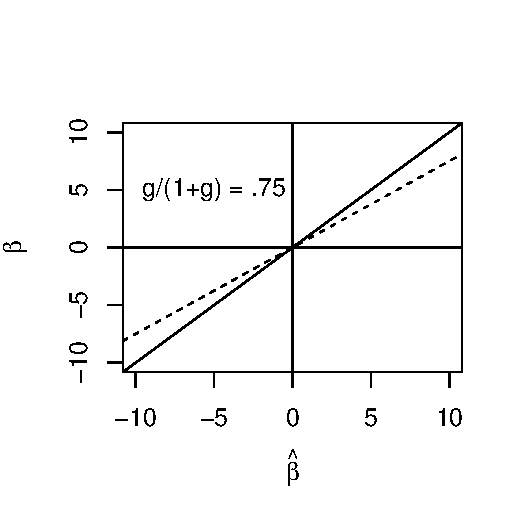
\includegraphics[width=\maxwidth]{figure/unnamed-chunk-1-1} 

\end{knitrout}




\end{frame}

\begin{frame}
  \frametitle{Jeffreys Prior}

Jeffreys proposed a default  procedure so that resulting prior
would be invariant to model parameterization  \pause

$$p(\t) \propto |\cI(\t)|^{1/2}$$
\pause
where $\cI(\t)$ is the  Expected Fisher Information matrix
\pause
$$
\cI(\theta) = - \E[ \left[ \frac{\partial^2 \log(\cL(\t))}{\partial
  \theta_i \partial \theta_j} \right] ]
$$
\end{frame}
\begin{frame}
  \frametitle{Fisher Information Matrix}
Log Likelihood
$$
    \log(\cL(\b, \phi))  =  \, \frac{n}{2} \log(\phi)  - \frac{\phi}{2}
     \| (\I - \P_\x) \Y\|^2
 - \frac{\phi}{2}(\b - \bhat)^T(\X^T\X)(\b - \bhat)
$$ \pause
  \begin{eqnarray*}
\frac{\partial^2 \log \cL} { \partial \t \partial \t^T} & = &
\left[
  \begin{array}{cc}
    -\phi (\X^T\X) & -(\X^T\X) (\b - \bhat) \\
  - (\b - \bhat)^T (\X^T\X) & -\frac{n}{2} \frac{1}{\phi^2} \\
  \end{array}
\right] \pause \\
\E[\frac{\partial^2 \log \cL} { \partial \t \partial \t^T}] & = &
\left[
  \begin{array}{cc}
    -\phi (\X^T\X) & \zero_p \\
  \zero_p^T & -\frac{n}{2} \frac{1}{\phi^2} \\
  \end{array}
\right] \pause \\
& & \\
\cI((\b, \phi)^T) & = & \left[
  \begin{array}{cc}
    \phi (\X^T\X) & \zero_p \\
  \zero_p^T & \frac{n}{2} \frac{1}{\phi^2}
  \end{array}
\right]
  \end{eqnarray*}
\end{frame}
\begin{frame}
  \frametitle{Jeffreys Prior}
  Jeffreys Prior
  \begin{eqnarray*}
  p_J(\b, \phi)  & \propto & |\cI((\b, \phi)^T) |^{1/2}   \pause \\
               & = & |\phi (\X^T\X|^{1/2} \left(\frac{n}{2}
                 \frac{1}{\phi^2} \right)^{1/2} \pause \\
  & \propto  &  \phi^{p/2 - 1} |\X^T\X|^{1/2} \pause \\
  & \propto & \phi^{p/2 - 1}  \pause
  \end{eqnarray*}
  Improper prior   $\iint p_J(\b, \phi) \, d\b \, d\phi $ not finite

\end{frame}
\begin{frame}
  \frametitle{Formal Bayes Posterior}
$$  p(\b, \phi \mid \Y) \propto p(\Y \mid \b, \phi)  \phi^{p/2 - 1} $$
\pause
if this is integrable, then renormalize to obtain formal posterior
distribution \pause


\begin{eqnarray*}
  \b \mid \phi, \Y & \sim & \N(\bhat, (\X^T\X)^{-1} \phi^{-1}) \\
  \phi \mid \Y & \sim& \G(n/2, \| \Y - \X\bhat \|^2/2)
\end{eqnarray*} \pause
Limiting case of Conjugate prior with $\bv_0 = 0$, $\Phi = \zero$,
$\nu_0 = 0$ and $\SS_0 = 0$ \pause

Posterior for $\phi$ does not depend on dimension $p$;   \pause

\vfill
Jeffreys did not recommend using this
\end{frame}
\begin{frame}
  \frametitle{Independent Jeffreys Prior "Reference Prior"}
  \begin{itemize}
  \item  Treat $\b$ and $\phi$ separately  (``orthogonal
    parameterization'') \pause
  \item $p_{IJ}(\b) \propto |\cI(\b)|^{1/2}$ \pause
\item $p_{IJ}(\phi) \propto |\cI(\phi)\|^{1/2}$ \pause
  \end{itemize}
$$
\cI((\b, \phi)^T)  =  \left[
  \begin{array}{cc}
    \phi (\X^T\X) & \zero_p \\
  \zero_p^T & \frac{n}{2} \frac{1}{\phi^2}
  \end{array}
\right]
$$
\pause
$$p_{IJ}(\b) \propto |\phi \X^T\X|^{1/2} \propto 1$$ \pause
$$p_{IJ}(\phi) \propto \phi^{-1}$$ \pause

Independent Jeffreys Prior is
$$p_{IJ}(\beta, \phi) \propto p_{IJ}(\b) p_{IJ}(\phi) = \phi^{-1}$$

\end{frame}
\begin{frame}
  \frametitle{Formal Posterior Distribution}
  With Independent Jeffreys Prior
$$p_{IJ}(\beta, \phi) \propto p_{IJ}(\b) p_{IJ}(\phi) = \phi^{-1}$$
\pause
Formal Posterior Distribution  (Show!)
\pause
\begin{eqnarray*}
  \b \mid \phi, \Y & \sim & \N(\bhat, (\X^T\X)^{-1} \phi^{-1}) \pause \\
  \phi \mid \Y & \sim& \G((n-p)/2, \| \Y - \X\bhat \|^2/2) \pause\\
\b \mid \Y & \sim & t_{n-p}(\bhat, \shat (\X^T\X)^{-1})\pause
\end{eqnarray*}
Bayesian Credible Sets
$p(\b \in C_\alpha) = 1- \alpha$ correspond to frequentist Confidence
Regions

$$\frac{\lambdab^T\b - \lambdab\bhat}
{\sqrt{\shat \lambdab^T(\X^T\X)^{-1} \lambdab}} \sim t_{n-p}$$

\end{frame}
\begin{frame}
  \frametitle{Disadvantages of Conjugate Priors}
  Disadvantages: \pause
\begin{itemize}
\item Results  may have be sensitive to the  prior mean which may appear as an ``outlier''  \pause
\vspace{1.5in}

\item Cannot capture all possible prior beliefs \pause
\item Mixtures of Conjugate Priors
\end{itemize}
\end{frame}

\begin{frame} \frametitle{Mixtures of Conjugate Priors}
  \begin{theorem}[Diaconis \& Ylivisaker 1985]  Given a sampling model
  $p(y \mid \t)$ from an exponential family, any prior distribution
  can be expressed as a mixture of conjugate prior distributions
 \end{theorem}

 \begin{itemize}
 \item Prior $p(\t) = \int p(\t \mid \omega) p(\omega)\, d \omega$ \pause
 \item Posterior \pause
   \begin{eqnarray*}
   p(\t \mid \Y)  &\propto & \int p(\Y \mid \t) p(\t \mid \omega)
   p(\omega) \, d\omega \pause \\
 & \propto & \int  \frac{  p(\Y \mid \t) p(\t \mid \omega) } {p(\Y \mid
   \omega)}  p(\Y \mid
 \omega) p(\omega ) \, d \omega  \pause \\
& \propto & \int p(\t \mid \Y, \omega)  p(\Y \mid
 \omega) p(\omega ) \, d \omega \pause \\
 p(\t \mid \Y) & =  & \frac{\int p(\t \mid \Y, \omega)  p(\Y \mid
 \omega) p(\omega ) \, d \omega }
{\int p(\Y \mid
 \omega) p(\omega ) \, d \omega }
       \end{eqnarray*}

 \end{itemize}
\end{frame}


\begin{frame} \frametitle{Zellner-Siow Cauchy Prior}

\begin{itemize}
\item Model $\Y \sim \N( \one \beta_0 + \X \b , \I_n\phi)$ and assume $\X^T\one = 0$  case where $X$ is centered and has mean 0
\item Conditional Zellner $g$ prior on $\b$
$$\b \mid g, \phi, \beta_0 \sim \N(0, g (\X^T\X)^{-1}/\phi)$$
\item Independent Jeffrey's prior on $\beta_0, \phi$
$$p(\beta_0, \phi \mid g) \propto 1/\phi$$

\item Gamma prior: $1/g \sim G(1/2, 1/2)$ $\Rightarrow$ Cauchy prior distribution
$$\b \mid  \phi, \beta_0 \sim C(0, g (\X^T\X)^{-1}/\phi)$$

\item Posterior Distributions
\begin{align*}
\beta_0 \mid \Y, \b, \phi, g & \sim N(\bar{Y}, \frac{1}{n \phi}) \\
\b \mid \Y, \phi, g  & \sim N( \frac{g}{1+g} \hat{\b},  \frac{g}{1+g} \frac{1}{\phi} (\X^T\X)^{-1} ) \\
\phi \mid \Y, g  & \sim G( , ) \\
g \mid \Y & \sim  ?
\end{align*}
\end{itemize}
\end{frame}
\end{document}

